
\chapter{El SAT como vacío de la intersección de una RCG con un lenguaje regular finito}
\label{cap:modelacion-sat}

Con la no linealidad de
las RCG se expresa la consistencia de cualquier fórmula, sin la
restricción sobre el orden de las ocurrencias presente en SATCF y
SATSRC. Esa modelación general es el punto de partida para buscar
restricciones no lineales con vacío tratable, y con ellas fragmentos
del SAT polinomiales más amplios que el de SATSRC.

En la sección~\ref{sec:modelacion-sat} se construye esa modelación y se
demuestra la reducción desde el SAT; en la sección~\ref{sec:lectura-sat} se lee
el resultado en términos del SAT y se desarrollan sus consecuencias.

\section{Modelación del SAT con RCG}
\label{sec:modelacion-sat}

A
una fórmula con $n$ ocurrencias de variable booleana se le asocian el autómata
booleano del capítulo~\ref{cap:rcg-sat}, finito y acíclico, y una RCG no
lineal\footnote{La consistencia se puede modelar con otras RCG no lineales; la que se
usa aquí es solo una propuesta.} que impone la consistencia entre las
ocurrencias de una misma variable booleana.

Sea $\ell_1\cdots\ell_n$ la secuencia de ocurrencias de la fórmula, con
$\ell_i$ la variable booleana de la ocurrencia $i$. Por ejemplo, la fórmula
$x_1 \wedge (x_2 \vee x_1)$ tiene la secuencia de ocurrencias
$x_1\,x_2\,x_1$, con $n = 3$, de modo que $\ell_1 = x_1$, $\ell_2 = x_2$
y $\ell_3 = x_1$. Las ocurrencias $1$ y $3$ son de la misma variable booleana
$x_1$.

La gramática de consistencia
$G_{\mathrm{cons}}$ tiene por terminales $T=\{0,1\}$, por variables
$X, W_0, W_1, \ldots, W_n$ y tres juegos de predicados, todos de
aridad uno: el predicado inicial $S$, un predicado $Eq_v$ por cada
variable booleana $v$ y los predicados $L_0, L_1, \ldots, L_n$. El
predicado $L_j$ reconoce las cadenas de longitud $j$, mediante las
cláusulas
\[
  L_j(cX) \to L_{j-1}(X) \quad (c \in \{0,1\},\ 1 \le j \le n),
  \qquad L_0(\varepsilon) \to \varepsilon.
\]
Por ejemplo, $L_3$ reconoce la cadena $101$ mediante la derivación
$L_3(101) \to L_2(01) \to L_1(1) \to L_0(\varepsilon) \to \varepsilon$,
que consume un símbolo en cada paso hasta llegar a la cadena vacía.

Para cada variable booleana $v$, con ocurrencias en las posiciones
$i_1 < i_2 < \cdots < i_r$, el predicado $Eq_v$ reconoce las cadenas de
longitud $n$ en las que esas posiciones llevan el mismo símbolo. Sus
cláusulas son dos, una por cada símbolo $b \in \{0,1\}$:
\[
  Eq_v(W_0\, b\, W_1\, b \cdots b\, W_r) \to
  L_{g_0}(W_0)\, L_{g_1}(W_1) \cdots L_{g_r}(W_r).
\]
Es decir, para cada variable booleana $v$ las dos cláusulas son
\[
\begin{aligned}
  Eq_v(W_0\, 0\, W_1\, 0 \cdots 0\, W_r) &\to
    L_{g_0}(W_0)\, L_{g_1}(W_1) \cdots L_{g_r}(W_r), \\
  Eq_v(W_0\, 1\, W_1\, 1 \cdots 1\, W_r) &\to
    L_{g_0}(W_0)\, L_{g_1}(W_1) \cdots L_{g_r}(W_r).
\end{aligned}
\]
En el argumento del lado izquierdo, el símbolo $b$ ocupa las posiciones de
$v$ y cada variable $W_k$ cubre una subcadena: la anterior a la primera
ocurrencia, la comprendida entre dos ocurrencias consecutivas o la
posterior a la última. Esas subcadenas tienen longitudes
$g_0 = i_1 - 1$, $g_k = i_{k+1} - i_k - 1$ y $g_r = n - i_r$, y cada
una se reconoce por el predicado $L_{g_k}$ correspondiente. Una vez
fijada la fórmula, las posiciones $i_k$ y las longitudes $g_k$ son
constantes, de modo que el conjunto de cláusulas es finito y cada
cláusula tiene la forma de la definición~\ref{def:rcg}. La
figura~\ref{fig:particion-eqv} ilustra esa partición para una variable
booleana con dos ocurrencias.

\begin{figure}[ht]
\centering
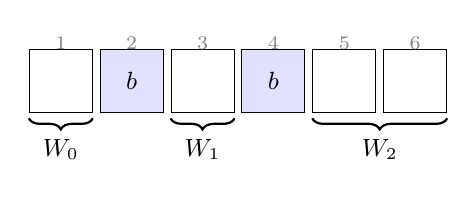
\begin{tikzpicture}[
    cell/.style={draw, minimum size=8mm, font=\small},
    bcell/.style={cell, fill=blue!12}]
  \node[cell]  (c1) at (0.9,0) {};
  \node[bcell] (c2) at (1.8,0) {$b$};
  \node[cell]  (c3) at (2.7,0) {};
  \node[bcell] (c4) at (3.6,0) {$b$};
  \node[cell]  (c5) at (4.5,0) {};
  \node[cell]  (c6) at (5.4,0) {};
  \foreach \i/\c in {1/c1, 2/c2, 3/c3, 4/c4, 5/c5, 6/c6}
    \node[font=\scriptsize, gray] at ([yshift=2pt]\c.north) {\i};
  \draw[decorate, decoration={brace, amplitude=4pt, mirror}, thick]
    ([yshift=-2pt]c1.south west) -- ([yshift=-2pt]c1.south east)
    node[midway, below=4pt, font=\small] {$W_0$};
  \draw[decorate, decoration={brace, amplitude=4pt, mirror}, thick]
    ([yshift=-2pt]c3.south west) -- ([yshift=-2pt]c3.south east)
    node[midway, below=4pt, font=\small] {$W_1$};
  \draw[decorate, decoration={brace, amplitude=4pt, mirror}, thick]
    ([yshift=-2pt]c5.south west) -- ([yshift=-2pt]c6.south east)
    node[midway, below=4pt, font=\small] {$W_2$};
\end{tikzpicture}
\caption[Partición del argumento de $Eq_v$]{Partición del argumento de $Eq_v$ para una variable booleana
$v$ con ocurrencias en las posiciones $i_1=2$ e $i_2=4$ de una cadena de
longitud $n=6$. Las celdas sombreadas llevan el símbolo $b$ en las
posiciones de $v$; cada $W_k$ cubre la subcadena entre ocurrencias
consecutivas, con longitudes $g_0=1$, $g_1=1$ y $g_2=2$.}
\label{fig:particion-eqv}
\end{figure}

La consistencia
de la fórmula es la conjunción\footnote{Por conjunción se entiende que
todas las restricciones deben cumplirse simultáneamente.} de esas
restricciones, y se expresa con
una cláusula no lineal con el mismo argumento en los $m$ predicados
$Eq_v$, donde $m$ es la cantidad de variables booleanas de la fórmula:
\[
  S(X) \to Eq_{v_1}(X)\, Eq_{v_2}(X) \cdots Eq_{v_m}(X).
\]
La variable $X$ es la misma en los $m$ predicados, así que las $m$
restricciones se aplican a la misma cadena. Con esta cláusula queda
completo el conjunto de cláusulas y, con él, la gramática
$G_{\mathrm{cons}}$. El lenguaje reconocido por $G_{\mathrm{cons}}$ se
denota $L(G_{\mathrm{cons}})$; el lema siguiente lo caracteriza.

\begin{lema}
\label{lema:lenguaje-gcons}
Sea $G_{\mathrm{cons}}$ la gramática de consistencia de una fórmula
booleana con $n$ ocurrencias de variable. El lenguaje
$L(G_{\mathrm{cons}})$ es el conjunto de las cadenas consistentes de
la fórmula.
\end{lema}

\begin{proof}
Primero se establece, por inducción sobre $j$, que $L_j(u)$ deriva en
la cadena vacía si y solo si $|u| = j$.

En el caso base, $j = 0$, la única cláusula con $L_0$ en el lado
izquierdo es $L_0(\varepsilon) \to \varepsilon$, que solo aplica cuando
el argumento es la cadena vacía; así, $L_0(u)$ deriva en la cadena
vacía si y solo si $u = \varepsilon$, esto es, $|u| = 0$.

En el paso inductivo, $j \ge 1$, se supone como hipótesis que
$L_{j-1}(u')$ deriva en la cadena vacía si y solo si $|u'| = j-1$. Las
únicas cláusulas con $L_j$ en el lado izquierdo son
$L_j(cX) \to L_{j-1}(X)$, con $c \in \{0,1\}$, de modo que $L_j(u)$
deriva en la cadena vacía solo si $u = c\,u'$ para algún símbolo $c$, y
la derivación continúa con $L_{j-1}(u')$. Entonces $L_j(u)$ deriva en
la cadena vacía si y solo si $L_{j-1}(u')$ lo hace, lo que por la
hipótesis equivale a $|u'| = j-1$; como $|u| = |u'| + 1$, esto equivale
a $|u| = j$.

Sea $w$ una cadena consistente; como lleva un símbolo por ocurrencia,
$|w| = n$. Para cada variable booleana $v$, sea $b$ el símbolo común
de sus posiciones en $w$. Entonces $w$ se descompone como
$u_0\, b\, u_1\, b \cdots b\, u_r$ con $|u_k| = g_k$: en el patrón
del símbolo $b$, la sustitución de rango asocia cada variable $W_k$ a
la subcadena $u_k$, y cada predicado $L_{g_k}(u_k)$ deriva en la
cadena vacía. Luego $Eq_v(w)$ deriva en la cadena vacía. Como esto
vale para las $m$ variables booleanas, con la cláusula de $S$ se
deriva en la cadena vacía y $w \in L(G_{\mathrm{cons}})$.

Sea ahora $w \in L(G_{\mathrm{cons}})$. La única cláusula de $S$ es
$S(X) \to Eq_{v_1}(X) \cdots Eq_{v_m}(X)$, de modo que cada $Eq_v(w)$
deriva en la cadena vacía. En esa derivación se aplica una de las dos
cláusulas de $Eq_v$, con algún símbolo $b$: entonces
$w = u_0\, b\, u_1\, b \cdots b\, u_r$, y cada predicado
$L_{g_k}(u_k)$ deriva en la cadena vacía, así que $|u_k| = g_k$. Como
$g_0 + g_1 + \cdots + g_r + r = n$ por la definición de las
longitudes $g_k$, se tiene $|w| = n$, y las posiciones
$i_1, \ldots, i_r$ de $w$ llevan el símbolo $b$. Como esto vale para
cada variable booleana, $w$ es consistente.
\end{proof}

Por ejemplo, considere la fórmula $x_1 \wedge (x_2 \vee x_1)$ del
capítulo~\ref{cap:rcg-sat}, cuya secuencia de ocurrencias es
$x_1\,x_2\,x_1$, con $n=3$ y $m=2$. La variable booleana $x_1$ ocurre en las
posiciones $1$ y $3$, con subcadenas de longitudes $g_0=0$, $g_1=1$ y
$g_2=0$; la variable booleana $x_2$ ocurre en la posición $2$, con subcadenas
de longitudes $g_0=1$ y $g_1=1$. Las cláusulas de $G_{\mathrm{cons}}$
son las siguientes, omitidas las de $L_2$ y $L_3$, que en ningún
patrón aparecen:
\[
\begin{aligned}
  S(X) &\to Eq_{x_1}(X)\, Eq_{x_2}(X),\\
  Eq_{x_1}(W_0\,0\,W_1\,0\,W_2) &\to L_0(W_0)\, L_1(W_1)\, L_0(W_2),\\
  Eq_{x_1}(W_0\,1\,W_1\,1\,W_2) &\to L_0(W_0)\, L_1(W_1)\, L_0(W_2),\\
  Eq_{x_2}(W_0\,0\,W_1) &\to L_1(W_0)\, L_1(W_1),\\
  Eq_{x_2}(W_0\,1\,W_1) &\to L_1(W_0)\, L_1(W_1),\\
  L_1(0X) \to L_0(X), \quad L_1(1X) &\to L_0(X), \qquad
  L_0(\varepsilon) \to \varepsilon.
\end{aligned}
\]

La figura~\ref{fig:particion-ejemplo} muestra, según la secuencia de
ocurrencias $x_1\,x_2\,x_1$, qué posiciones cubre cada $W_k$ en los
patrones de $Eq_{x_1}$ y $Eq_{x_2}$.

\begin{figure}[ht]
\centering
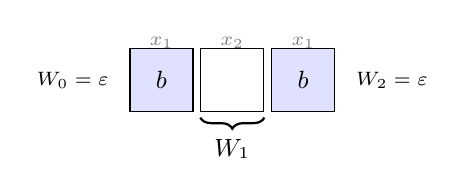
\begin{tikzpicture}[
    cell/.style={draw, minimum size=8mm, font=\small},
    bcell/.style={cell, fill=blue!12}]
  \node[bcell] (a1) at (0.9,0) {$b$};
  \node[cell]  (a2) at (1.8,0) {};
  \node[bcell] (a3) at (2.7,0) {$b$};
  \foreach \t/\c in {x_1/a1, x_2/a2, x_1/a3}
    \node[font=\scriptsize, gray] at ([yshift=2pt]\c.north) {$\t$};
  \node[font=\scriptsize, anchor=east] at ([xshift=-4pt]a1.west) {$W_0=\varepsilon$};
  \node[font=\scriptsize, anchor=west] at ([xshift=4pt]a3.east) {$W_2=\varepsilon$};
  \draw[decorate, decoration={brace, amplitude=4pt, mirror}, thick]
    ([yshift=-2pt]a2.south west) -- ([yshift=-2pt]a2.south east)
    node[midway, below=4pt, font=\small] {$W_1$};
\end{tikzpicture}

{\small (a) patrón de $Eq_{x_1}$: las posiciones $1$ y $3$ llevan $b$}

\vspace{1em}

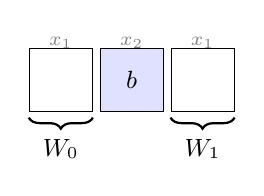
\begin{tikzpicture}[
    cell/.style={draw, minimum size=8mm, font=\small},
    bcell/.style={cell, fill=blue!12}]
  \node[cell]  (b1) at (0.9,0) {};
  \node[bcell] (b2) at (1.8,0) {$b$};
  \node[cell]  (b3) at (2.7,0) {};
  \foreach \t/\c in {x_1/b1, x_2/b2, x_1/b3}
    \node[font=\scriptsize, gray] at ([yshift=2pt]\c.north) {$\t$};
  \draw[decorate, decoration={brace, amplitude=4pt, mirror}, thick]
    ([yshift=-2pt]b1.south west) -- ([yshift=-2pt]b1.south east)
    node[midway, below=4pt, font=\small] {$W_0$};
  \draw[decorate, decoration={brace, amplitude=4pt, mirror}, thick]
    ([yshift=-2pt]b3.south west) -- ([yshift=-2pt]b3.south east)
    node[midway, below=4pt, font=\small] {$W_1$};
\end{tikzpicture}

{\small (b) patrón de $Eq_{x_2}$: la posición $2$ lleva $b$}
\caption[Subcadenas cubiertas por cada $W_k$]{Subcadenas que cubre cada $W_k$ sobre la secuencia de
ocurrencias $x_1\,x_2\,x_1$. La fila superior indica a qué variable
booleana pertenece cada posición. En (a), para $Eq_{x_1}$, las posiciones $1$ y $3$ son de
$x_1$ y $W_1$ cubre la posición $2$, con $W_0$ y $W_2$ vacías
($g_0=g_2=0$, $g_1=1$). En (b), para $Eq_{x_2}$, la posición $2$ es de
$x_2$ y $W_0$, $W_1$ cubren las posiciones $1$ y $3$ ($g_0=g_1=1$).}
\label{fig:particion-ejemplo}
\end{figure}

La cadena $101$ es consistente y se reconoce por $G_{\mathrm{cons}}$
mediante las derivaciones siguientes:
\[
\begin{aligned}
  S(101) &\to Eq_{x_1}(101)\, Eq_{x_2}(101),\\
  Eq_{x_1}(101) &\to L_0(\varepsilon)\, L_1(0)\, L_0(\varepsilon),\\
  Eq_{x_2}(101) &\to L_1(1)\, L_1(1),\\
  L_1(0) &\to L_0(\varepsilon),\\
  L_1(1) &\to L_0(\varepsilon),\\
  L_0(\varepsilon) &\to \varepsilon.
\end{aligned}
\]
A continuación se describen los pasos.
\begin{itemize}
  \item \textbf{Primer paso:} en la cláusula
    $S(X) \to Eq_{x_1}(X)\, Eq_{x_2}(X)$, la sustitución de rango
    asocia la variable $X$ al valor $X = 101$. De esta forma se deriva
    en $Eq_{x_1}(101)\, Eq_{x_2}(101)$.
  \item \textbf{Segundo paso:} en el patrón del símbolo $1$ de
    $Eq_{x_1}$, la sustitución de rango asocia las variables $W_0$,
    $W_1$, $W_2$ a los valores $W_0 = \varepsilon$, $W_1 = 0$ y
    $W_2 = \varepsilon$. Con estos valores se deriva en
    $L_0(\varepsilon)\, L_1(0)\, L_0(\varepsilon)$.
  \item \textbf{Tercer paso:} en el patrón del símbolo $0$ de
    $Eq_{x_2}$, la sustitución de rango asocia las variables $W_0$,
    $W_1$ a los valores $W_0 = 1$ y $W_1 = 1$. Con estos valores se
    deriva en $L_1(1)\, L_1(1)$.
  \item \textbf{Cuarto paso:} cada predicado $L_1$ deriva en
    $L_0(\varepsilon)$, y cada predicado $L_0(\varepsilon)$ deriva en
    la cadena vacía por la cláusula terminal, con lo que la cadena
    $101$ queda reconocida y $101 \in L(G_{\mathrm{cons}})$.
\end{itemize}

La figura~\ref{fig:arbol-derivacion-101} muestra el árbol de derivación
completo de $101$ en $G_{\mathrm{cons}}$.

\begin{figure}[ht]
\centering
\begin{forest}
for tree={font=\footnotesize, parent anchor=south, child anchor=north,
          l sep=7mm, s sep=3mm, inner sep=2pt}
[$S(101)$
  [$Eq_{x_1}(101)$
    [$L_0(\varepsilon)$ [$\varepsilon$]]
    [$L_1(0)$ [$L_0(\varepsilon)$ [$\varepsilon$]]]
    [$L_0(\varepsilon)$ [$\varepsilon$]]
  ]
  [$Eq_{x_2}(101)$
    [$L_1(1)$ [$L_0(\varepsilon)$ [$\varepsilon$]]]
    [$L_1(1)$ [$L_0(\varepsilon)$ [$\varepsilon$]]]
  ]
]
\end{forest}
\caption[Árbol de derivación de $101$ en $G_{\mathrm{cons}}$]{Árbol de derivación de la cadena $101$ en $G_{\mathrm{cons}}$.
Los hijos de cada nodo son los predicados del lado derecho de la
cláusula que se le aplica; las hojas $\varepsilon$ corresponden a la
cláusula terminal $L_0(\varepsilon) \to \varepsilon$.}
\label{fig:arbol-derivacion-101}
\end{figure}

La cadena $110$, con la que en el capítulo~\ref{cap:rcg-sat} se llega
al estado $V$ del autómata booleano, no es consistente. En
$Eq_{x_1}(110)$ ningún patrón admite una sustitución de rango: el del
símbolo $0$ exige $0$ en la posición $1$, donde la cadena lleva $1$, y
el del símbolo $1$ exige $1$ en la posición $3$, donde la cadena lleva
$0$.
Como $Eq_{x_1}(110)$ no deriva en la cadena vacía,
$110 \notin L(G_{\mathrm{cons}})$. La
figura~\ref{fig:no-consistencia-110} lo ilustra.

\begin{figure}[ht]
\centering
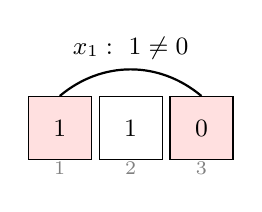
\begin{tikzpicture}[
    cell/.style={draw, minimum size=8mm, font=\small},
    xcell/.style={cell, fill=red!12}]
  \node[xcell] (c1) at (0.9,0) {$1$};
  \node[cell]  (c2) at (1.8,0) {$1$};
  \node[xcell] (c3) at (2.7,0) {$0$};
  \foreach \i/\c in {1/c1, 2/c2, 3/c3}
    \node[font=\scriptsize, gray] at ([yshift=-3pt]\c.south) {\i};
  \draw[thick] (c1.north) to[bend left=40]
       node[above, font=\small] {$x_1:\ 1 \ne 0$} (c3.north);
\end{tikzpicture}
\caption[La cadena $110$ no es consistente]{La cadena $110$ no es consistente: las dos ocurrencias de
$x_1$ (posiciones $1$ y $3$, sombreadas) llevan símbolos distintos.}
\label{fig:no-consistencia-110}
\end{figure}

La correctitud de esta modelación se demuestra en el teorema
siguiente.

\begin{teorema}
\label{teo:sat-vacio-interseccion}
Sean $G_{\mathrm{cons}}$ la gramática de consistencia de una fórmula
booleana y $A$ su autómata booleano. La fórmula es satisfacible si y
solo si $L(G_{\mathrm{cons}}) \cap L(A) \neq \emptyset$.
\end{teorema}

\begin{proof}
El lenguaje del autómata booleano está formado por las cadenas para
las que la fórmula es verdadera cuando cada ocurrencia se trata por
separado~\cite{fernandezarias2007}.

A cada interpretación $I$ de la fórmula le corresponde la cadena
$w_I = b_1 b_2 \cdots b_n$, de longitud $n$, el número de ocurrencias
de variable booleana de la fórmula. Cada $b_i$ es $1$ si $\ell_i$, la variable booleana de la ocurrencia
$i$, es verdadera en $I$, y $0$ si es falsa. La cadena $w_I$ es consistente: cada variable booleana tiene un único
valor en $I$, así que todas sus posiciones en $w_I$ llevan ese mismo
valor. Recíprocamente, toda cadena consistente es $w_I$ para la
interpretación $I$ en la que cada variable booleana toma el símbolo
común de sus posiciones.

Supóngase que la fórmula es satisfacible. Entonces la fórmula es
verdadera en alguna interpretación $I$. La cadena $w_I$ es consistente,
de modo que $w_I \in L(G_{\mathrm{cons}})$ por el
lema~\ref{lema:lenguaje-gcons}, y $w_I \in L(A)$. Luego la
intersección es no vacía.

Supóngase ahora que la intersección es no vacía. Entonces alguna
cadena $w$ pertenece a $L(G_{\mathrm{cons}})$ y a $L(A)$. Por el
lema~\ref{lema:lenguaje-gcons}, $w$ es consistente, de modo que
$w = w_I$ para la interpretación $I$ en la que cada variable booleana
toma el símbolo común de sus posiciones. De $w_I \in L(A)$ se sigue que
la fórmula es verdadera en $I$. Por tanto, la fórmula es satisfacible.
\end{proof}

El SAT se reduce entonces al problema de vacío de la intersección que
se resuelve en el capítulo~\ref{cap:vacio-interseccion-rcg-regular}. A
continuación se lee esta reducción en términos del SAT y se desarrollan
sus consecuencias.

\section{Consecuencias para el SAT y subclases tratables}
\label{sec:lectura-sat}

En la enumeración del capítulo~\ref{cap:vacio-interseccion-rcg-regular}
se recorren las cadenas aceptadas por el autómata booleano y se aplica
a cada una el reconocimiento de la RCG de consistencia; las dos partes
de la instancia tienen costo polinomial. El autómata booleano tiene
$O(n^2)$ estados, con $n$ la cantidad de
ocurrencias de variables booleanas en la fórmula~\cite{fernandezarias2007}. La gramática
$G_{\mathrm{cons}}$ tiene tamaño $O(m + n)$, con $m$ la cantidad de
variables booleanas distintas: dos cláusulas por variable booleana, más
las $O(n)$ cláusulas de los predicados $L_j$. Como $m \le n$, ese tamaño
es $O(n)$. El reconocimiento con
$G_{\mathrm{cons}}$ es polinomial: para cada cadena hay a lo sumo una
sustitución de rango por cláusula, porque los rangos de las variables
$W_k$ se determinan a partir de las longitudes $g_k$, y esa sustitución
se comprueba
en tiempo lineal; el reconocimiento de una cadena de longitud $n$
cuesta entonces $R_{G_{\mathrm{cons}}}(n) = O(nm)$.

Toda cadena aceptada por el autómata booleano tiene longitud $n$, de
modo que cada llamada a $\proc{RCG-Recognize}$ cuesta $O(nm)$. Con
$|Q| = O(n^2)$, la cota de la
subsección~\ref{sec:complejidad-algoritmo} queda en
\[
  O\bigl( n^2 + p(A)\,(n^2 + nm) \bigr) = O\bigl( n^2 + p(A)\,n^2 \bigr),
\]
pues $m \le n$. El factor dominante es $p(A)$, la cantidad de cadenas
aceptadas por el autómata booleano, que para una fórmula con muchas
interpretaciones verdaderas bajo el supuesto de independencia es del
orden de $2^n$. En el peor caso, la cota queda en
\[
  O\bigl( n^2 + 2^n\, n^2 \bigr) = O\bigl( 2^n\, n^2 \bigr).
\]
La dificultad no está entonces en el tamaño de la
instancia ni en el reconocimiento, sino en el vacío de la intersección: decidir si
$L(G_{\mathrm{cons}}) \cap L(A)$ es vacío es el SAT, y para una RCG
con un autómata finito acíclico ese problema es
NP-completo~\cite{bertsch2001rcg}.

De esta modelación se siguen tres consecuencias para el SAT. Con ella
y la enumeración del capítulo~\ref{cap:vacio-interseccion-rcg-regular}
se decide la satisfacibilidad de cualquier fórmula booleana, sin la
restricción de orden de SATCF y SATSRC. El alcance es general, pero la
decisión es por fuerza bruta: el costo es exponencial, y solo es
polinomial cuando el autómata booleano tiene una cantidad de caminos
aceptantes acotada por un polinomio en $n$; aquí no se caracterizan
las fórmulas booleanas que cumplen esa condición. La gramática de consistencia tiene aridad uno: con la
no linealidad, la aridad de las cláusulas no crece con los cruces. En
SATSRC el vacío de la intersección se decide en tiempo $O(n^k)$, con
$k$ la aridad: el exponente crece con la aridad necesaria para los
cruces, y la cota deja de ser polinomial cuando esa aridad no está
acotada. Con la no linealidad la aridad se mantiene en uno, a costa de
que el vacío de la intersección sea NP-completo. Por
último, la modelación es una propuesta concreta de cómo expresar el
SAT con una RCG. Con un procedimiento polinomial para el vacío de la intersección
de una RCG con un autómata acíclico se decidiría el SAT en tiempo
polinomial, esto es, $P = NP$. Con una subclase no lineal cuyo vacío de la intersección sea
polinomial se obtendría, en cambio, un fragmento tratable; pero esta
modelación se beneficiaría de esa tratabilidad solo si su gramática de
consistencia pertenece a la subclase, y, si no, sirve únicamente como
guía para adaptar la construcción a una subclase de ese tipo, sin
garantía de que sea posible.

En este capítulo se modeló el SAT como el vacío de la intersección de
una RCG con un lenguaje regular finito: a cada fórmula booleana se le
asociaron un autómata booleano y una RCG de consistencia no lineal, se
demostró la reducción desde el SAT y se leyeron sus consecuencias.
Para estudiar ese vacío hace falta una
representación simbólica de la intersección. En el próximo capítulo se
construye una: la gramática producto entre una RCG y un lenguaje
regular; con ella el problema general no se vuelve polinomial, pero se
obtiene el objeto sobre el que estudiar ese vacío: buscar subclases no
lineales con vacío polinomial, un algoritmo polinomial para el caso
general o argumentos de que no existe.

